\documentclass[12pt, a4paper]{article}
\usepackage {etex}
\usepackage{amsmath,amsfonts,amssymb,amsthm,mathtools}  
\usepackage{leqno}
\usepackage{fontspec}         
\defaultfontfeatures{Mapping=tex-text}
\newfontfamily{\cyrillicfont}{Arial}


\usepackage{unicode-math}     
\setmathfont{Asana-Math.otf}

\usepackage{polyglossia}      
\setdefaultlanguage{russian} 
\setotherlanguage{english} 
\usepackage{graphicx}                  
\usepackage{graphics}
\graphicspath{{images/}{pictures/}}    
\usepackage{wrapfig}                   
\usepackage{subfigure} 
\usepackage{tabularx}            
\usepackage{tabulary}          
\usepackage{array}               
\usepackage{longtable}           
\usepackage{multirow}            
\usepackage{float}               
\usepackage{booktabs}             
\usepackage{caption}
\renewcommand{\arraystretch}{1.3} 

\title{Pop art}
\author{Дарина }

\begin{document}
\maketitle
\begin{figure}[H]

\begin{minipage}[H]{0.32\linewidth} 
 \center 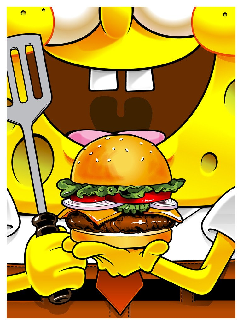
\includegraphics[width= 3.1 cm]{pop8.pdf}
\end{minipage}\hfill
\begin{minipage}[H]{0.32\linewidth} 
\center \includegraphics[width= 3.25 cm ]{pop5.pdf}
\end{minipage}\hfill
\begin{minipage}[H]{0.32\linewidth} 
\center 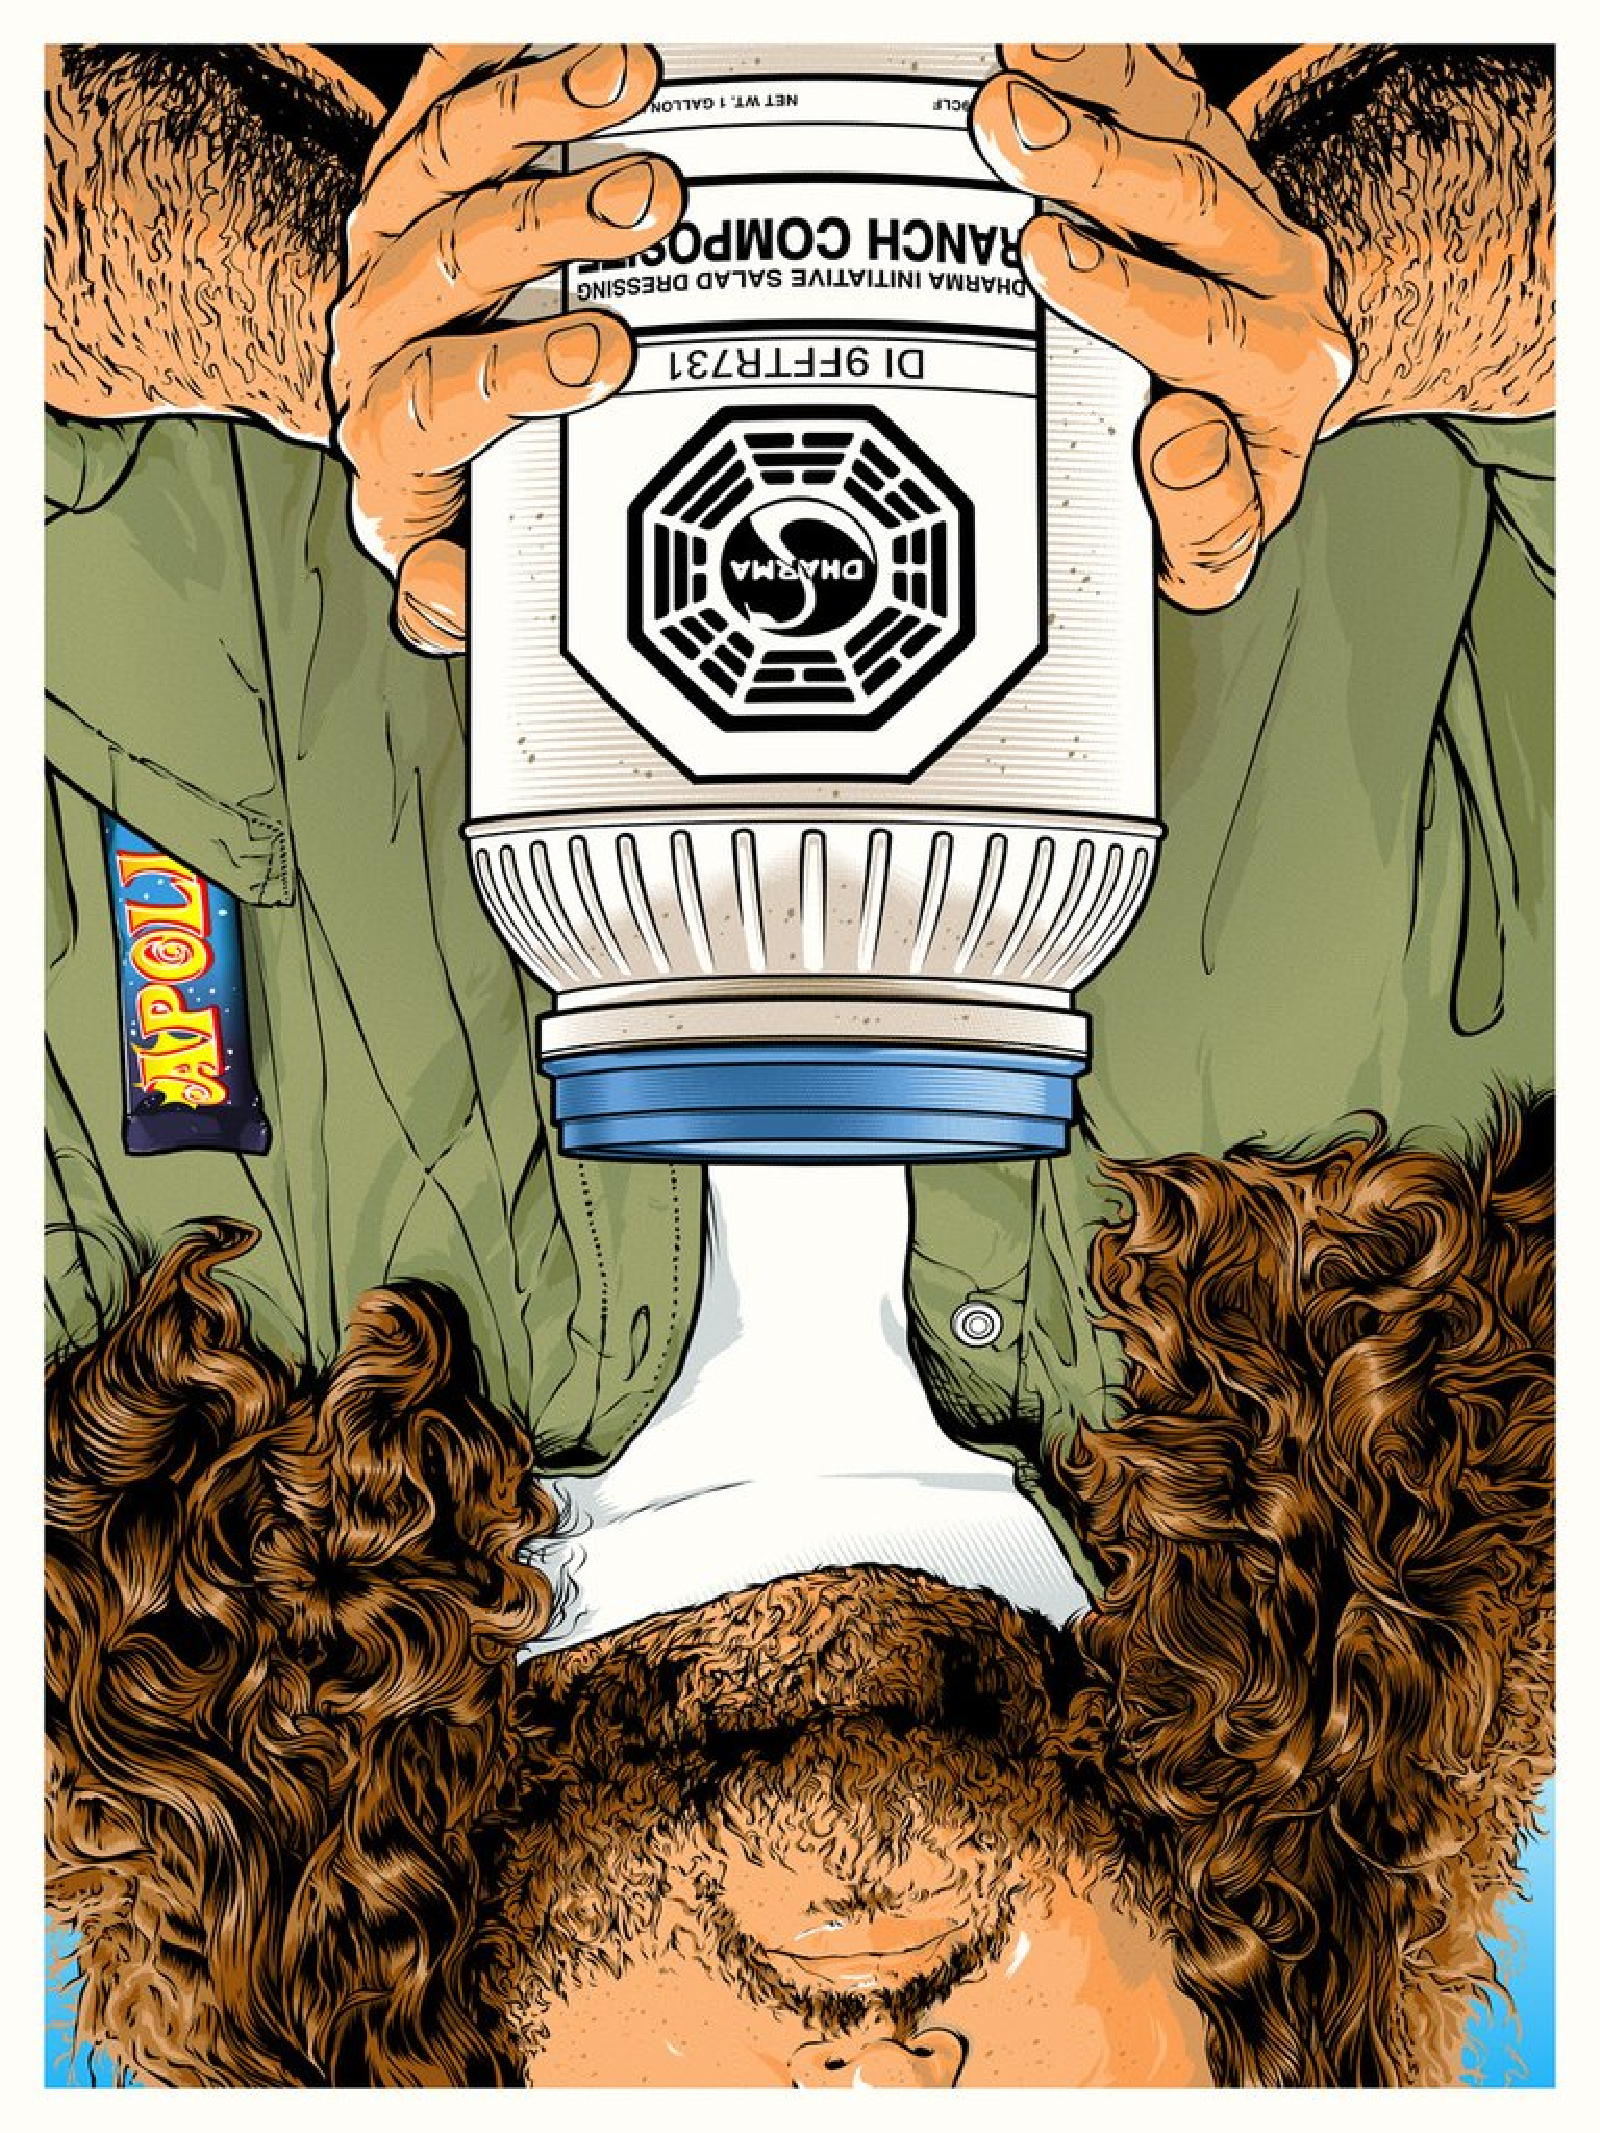
\includegraphics[width= 3.3 cm, angle = 180 ]{pop10.pdf}
\end{minipage}\vfill
\begin{minipage}[H]{0.32\linewidth} 
 \center 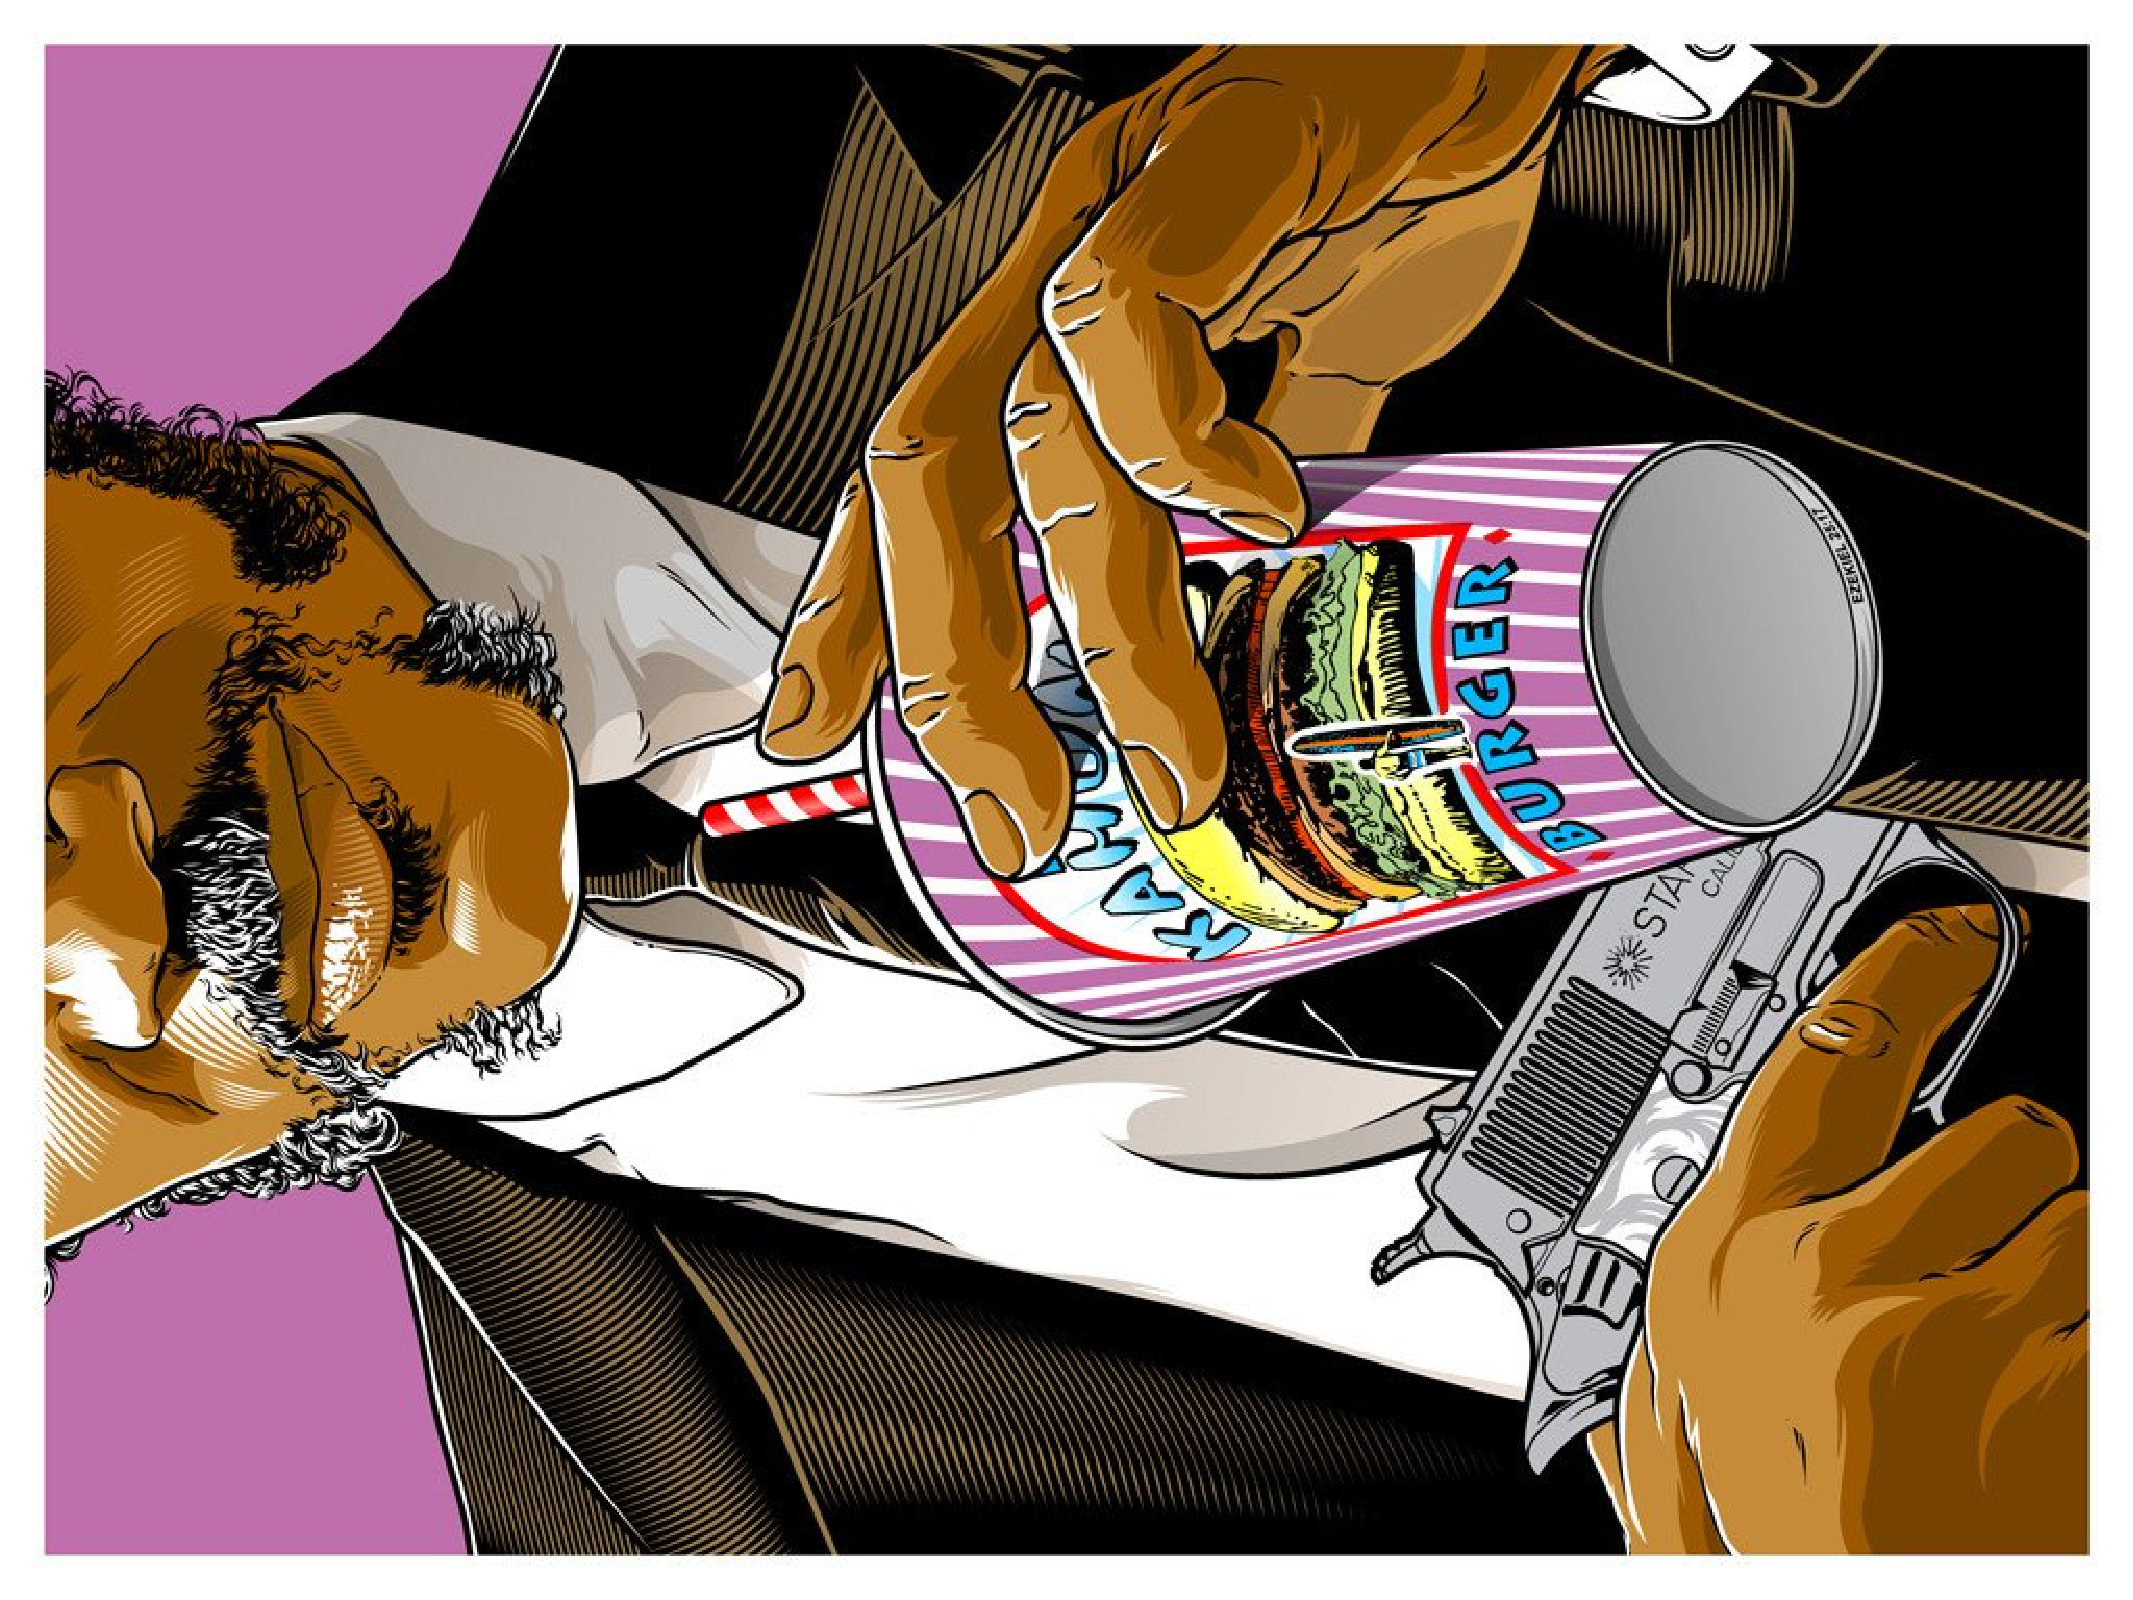
\includegraphics[angle = 270, width= 3.2 cm]{pop1.pdf}
\end{minipage}\hfill
\begin{minipage}[H]{0.32\linewidth} 
\center 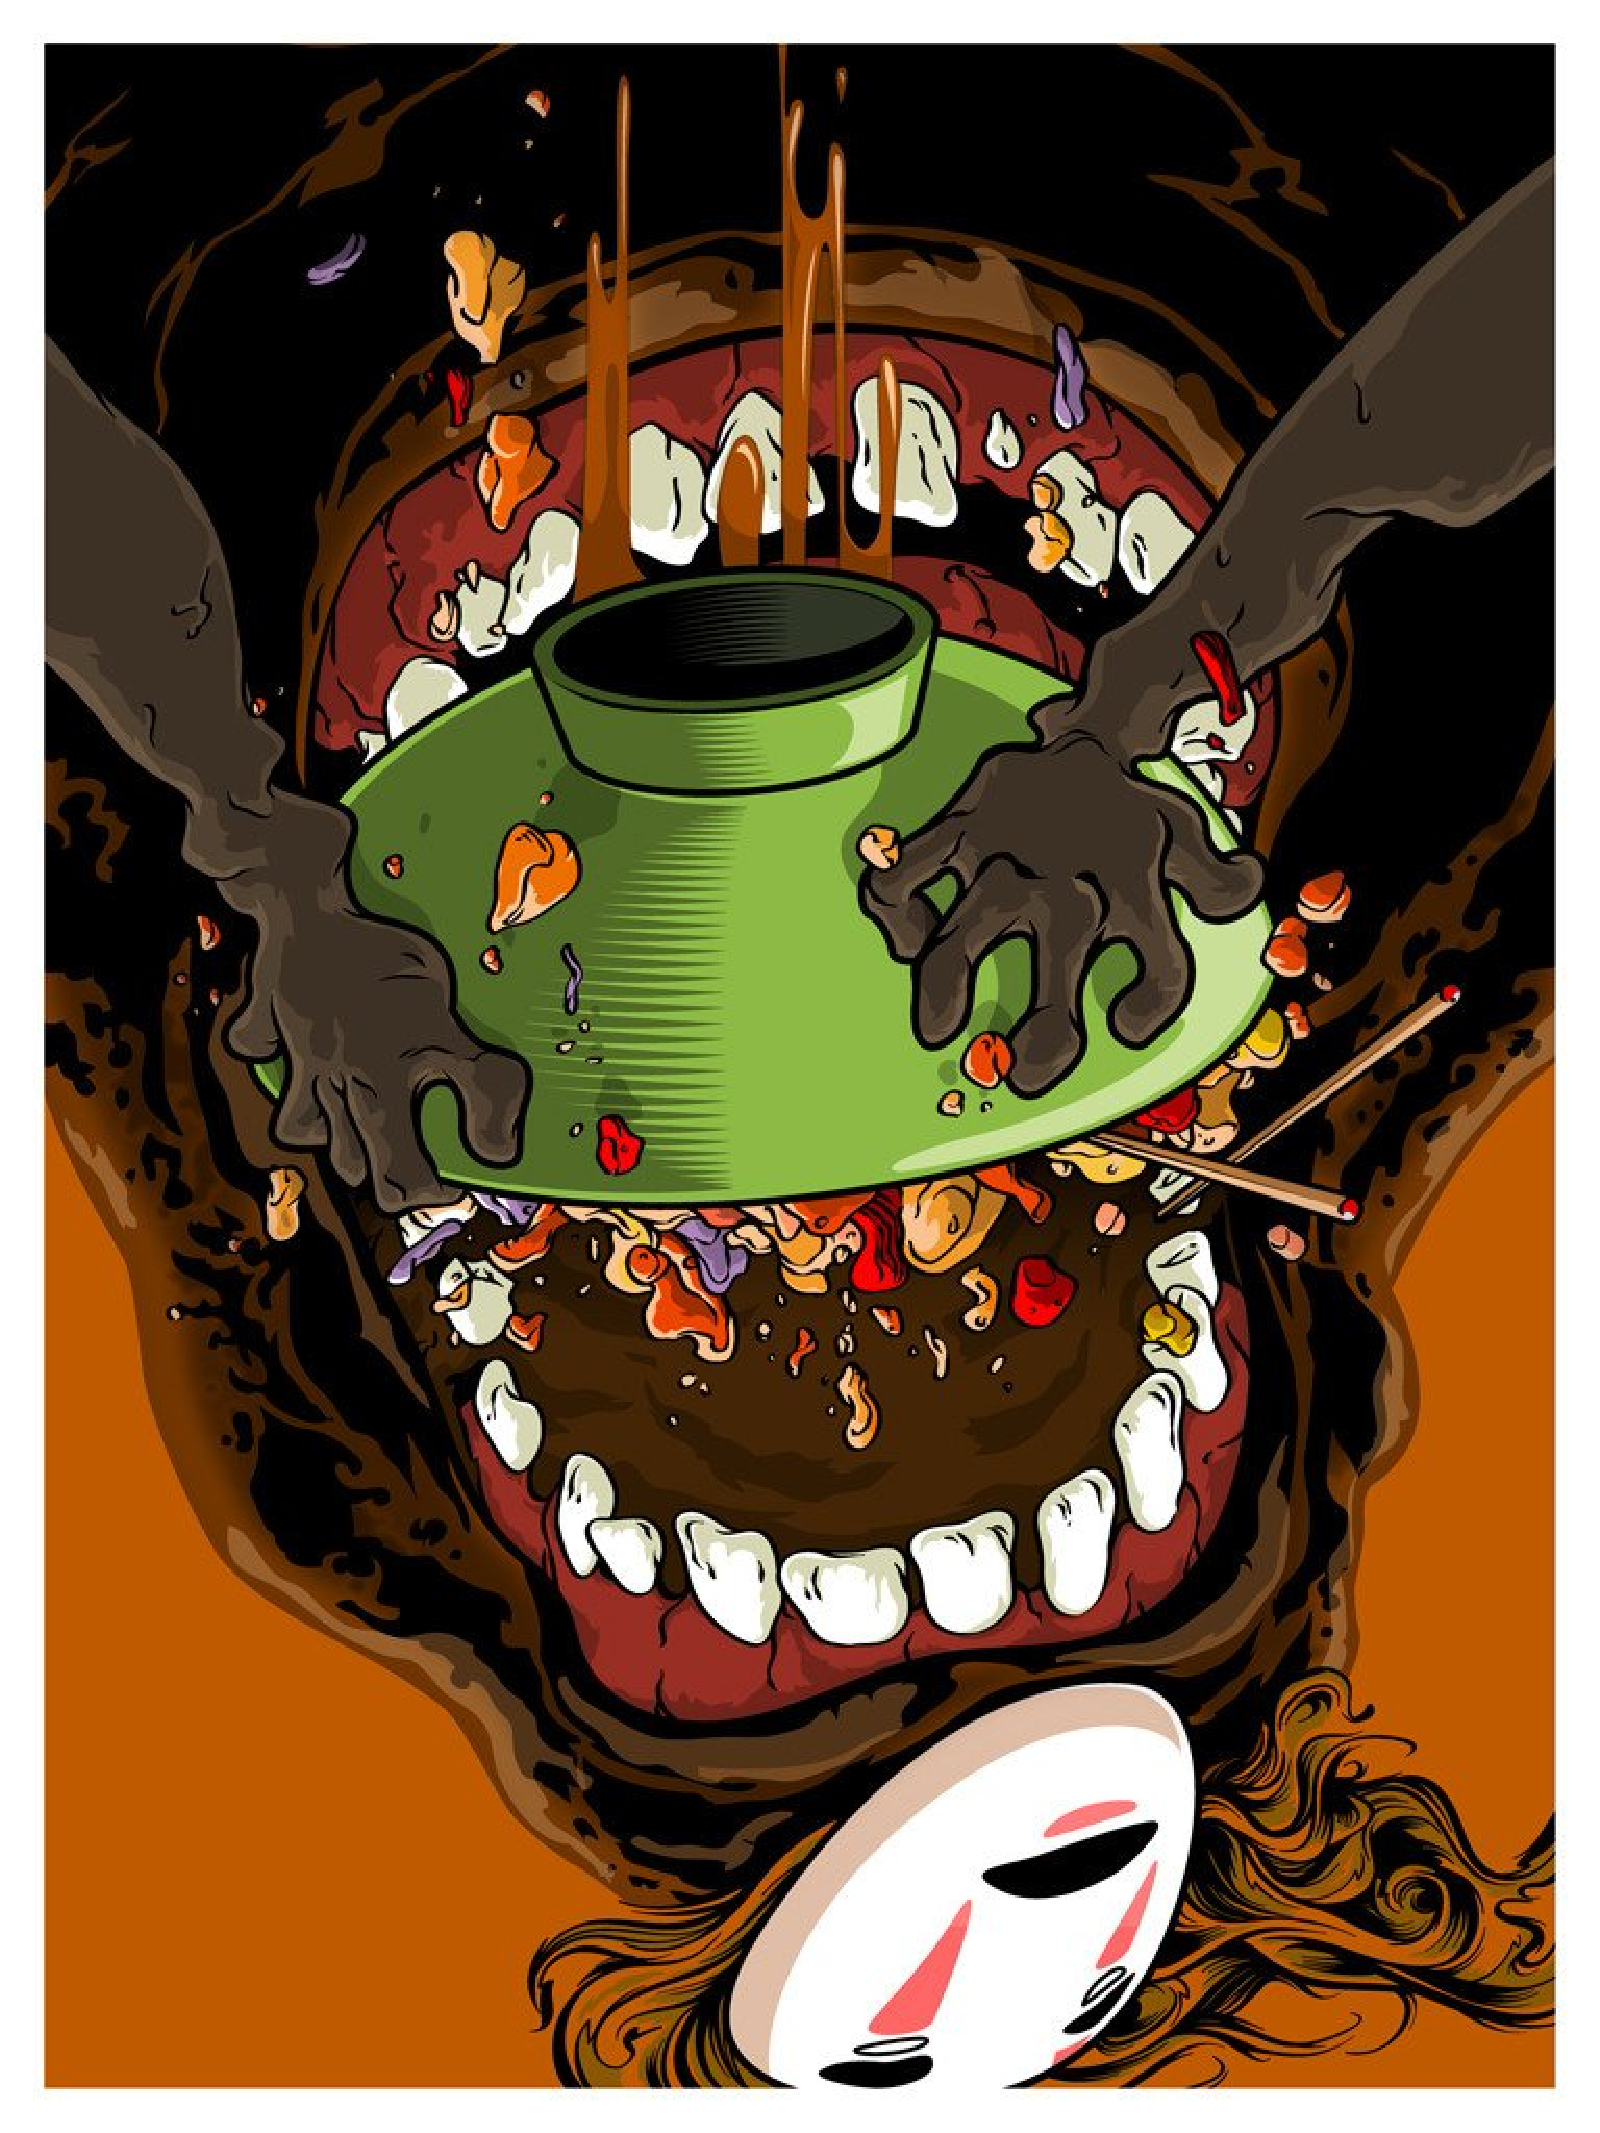
\includegraphics[width= 3.3 cm, angle = 180 ]{pop6.pdf}
\end{minipage}\hfill
\begin{minipage}[H]{0.32\linewidth} 
 \center 
\includegraphics[width= 3.1 cm]{pop3.pdf}
\end{minipage}
\caption {Это что, поп-арт?}
\end{figure}



\newpage
\begin{table}[H]
\begin{center}
\begin{tabular}{ m{5 cm}  m{3.5 cm} m{3.5 cm} }

 \begin{center} 
\includegraphics[width= 3.5 cm, angle =45, height= 4.6 cm]{pop4.pdf} \end{center}
 
 &\begin{center} \includegraphics[width= 2.1 cm ]{pop5.pdf} \end{center}
 
& \begin{center}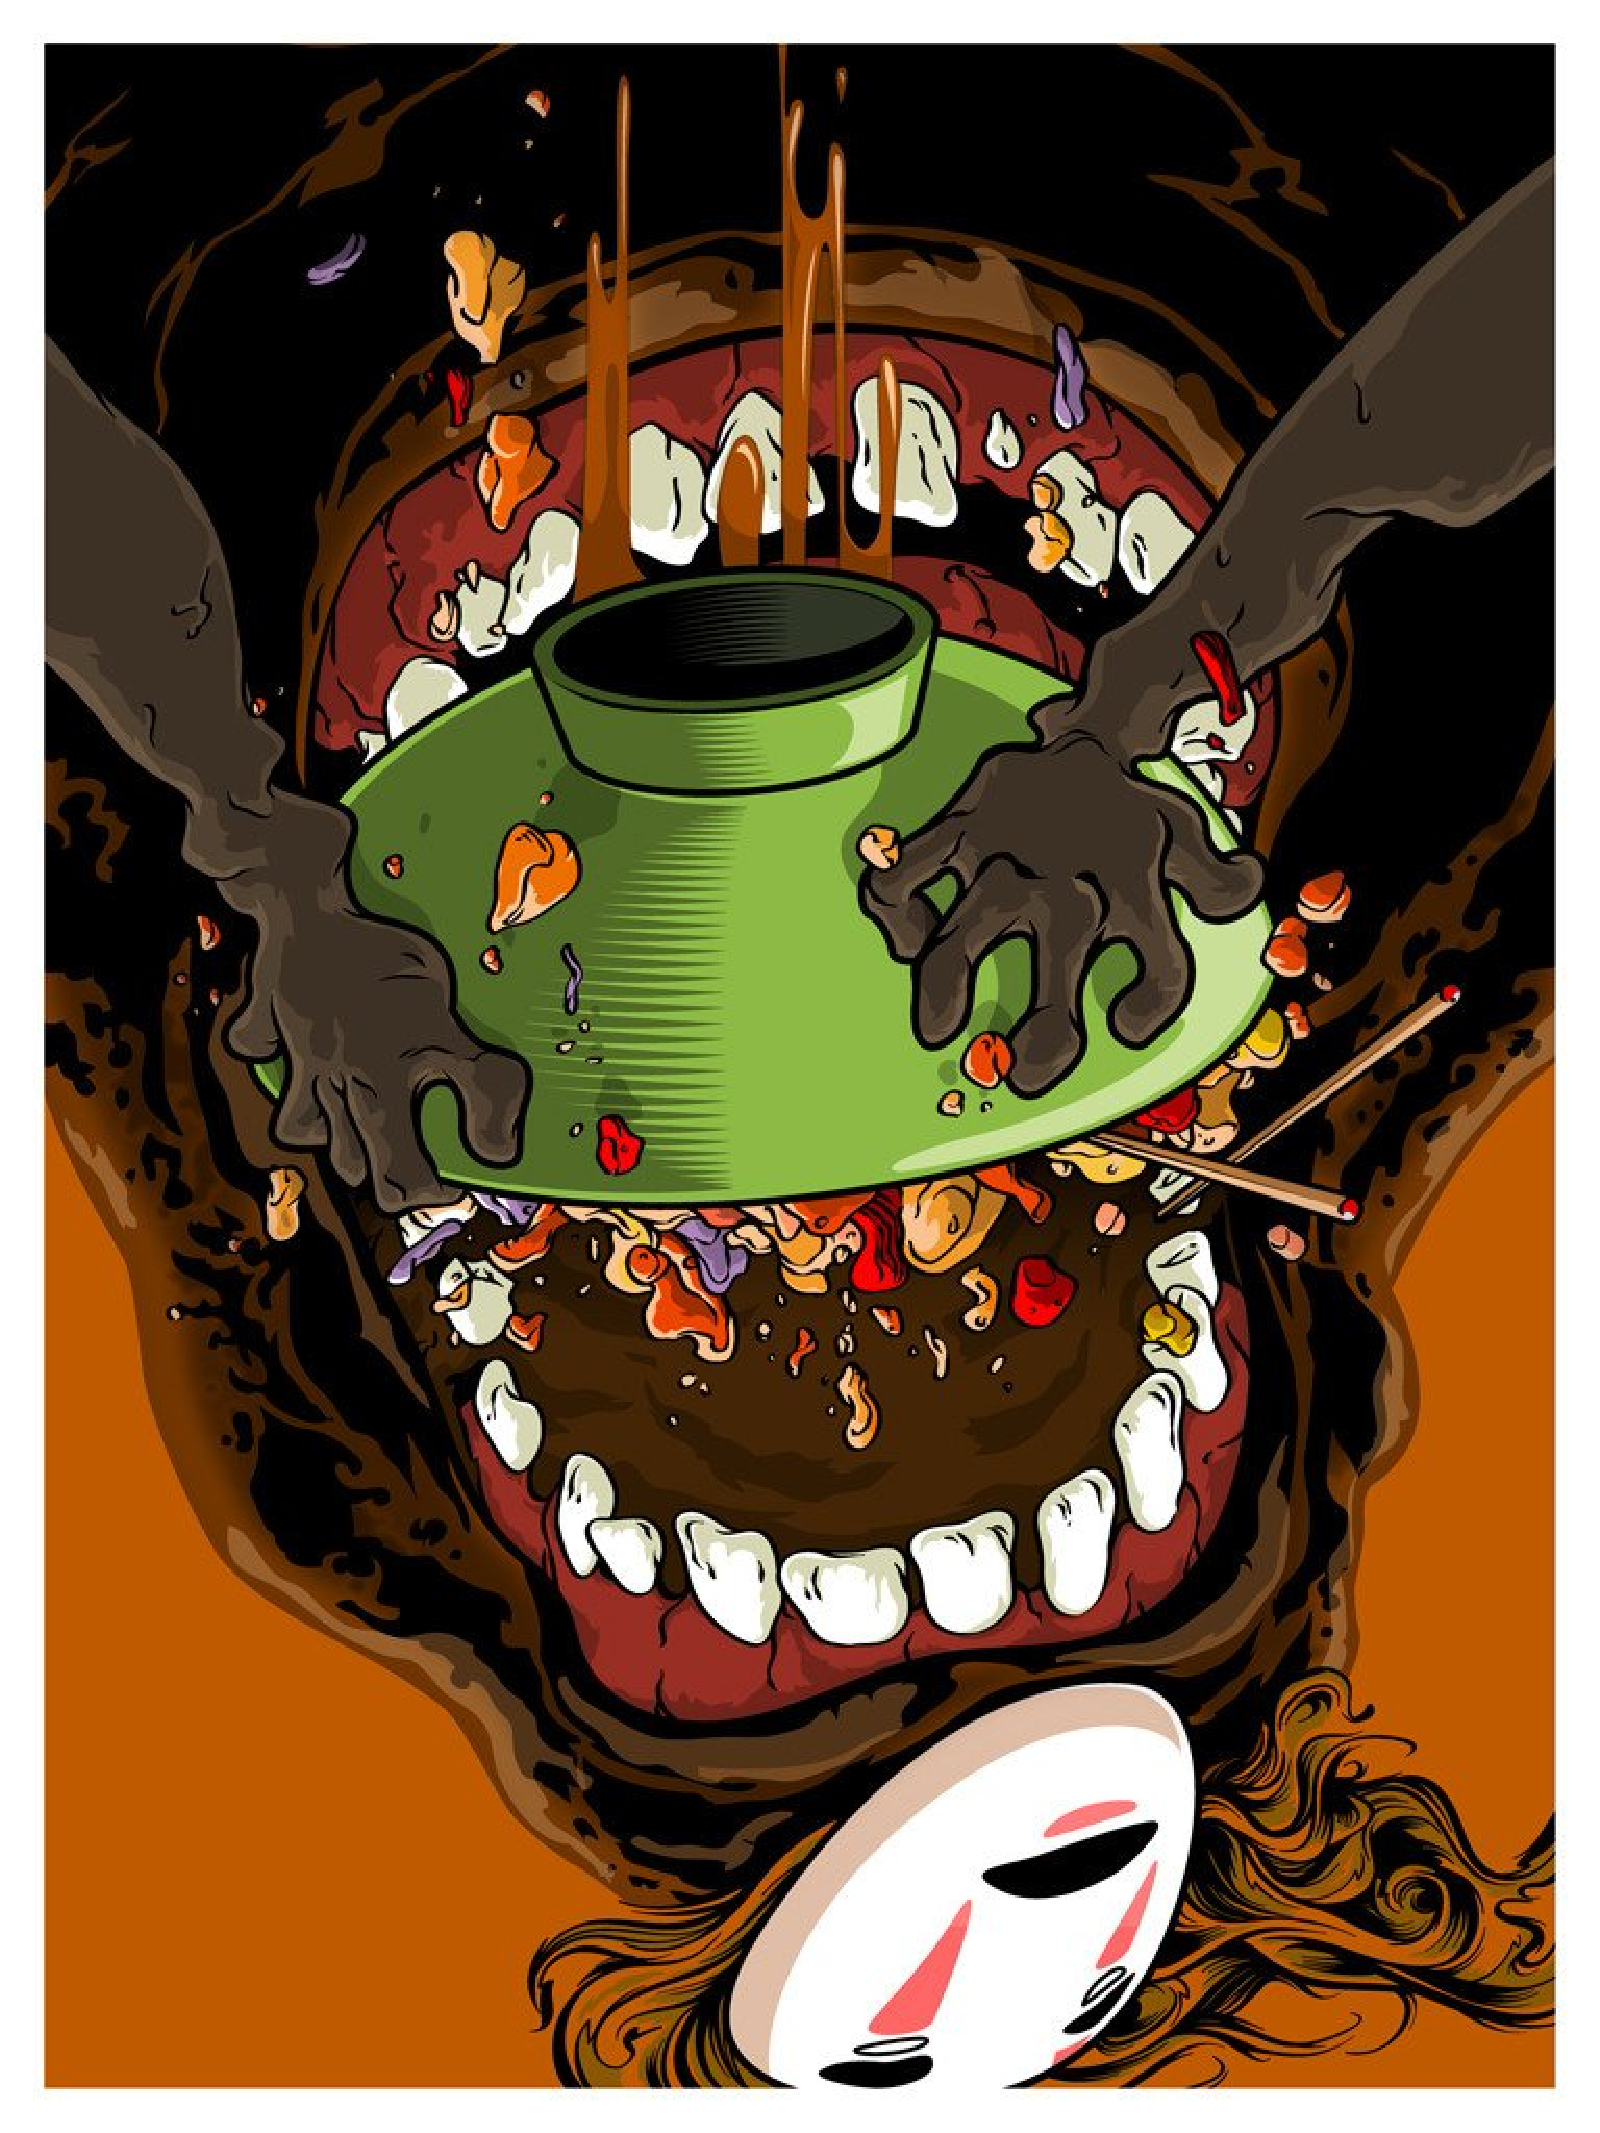
\includegraphics[width= 2.1 cm, angle = 180]{pop6.pdf} \end{center} \\

\begin{center} 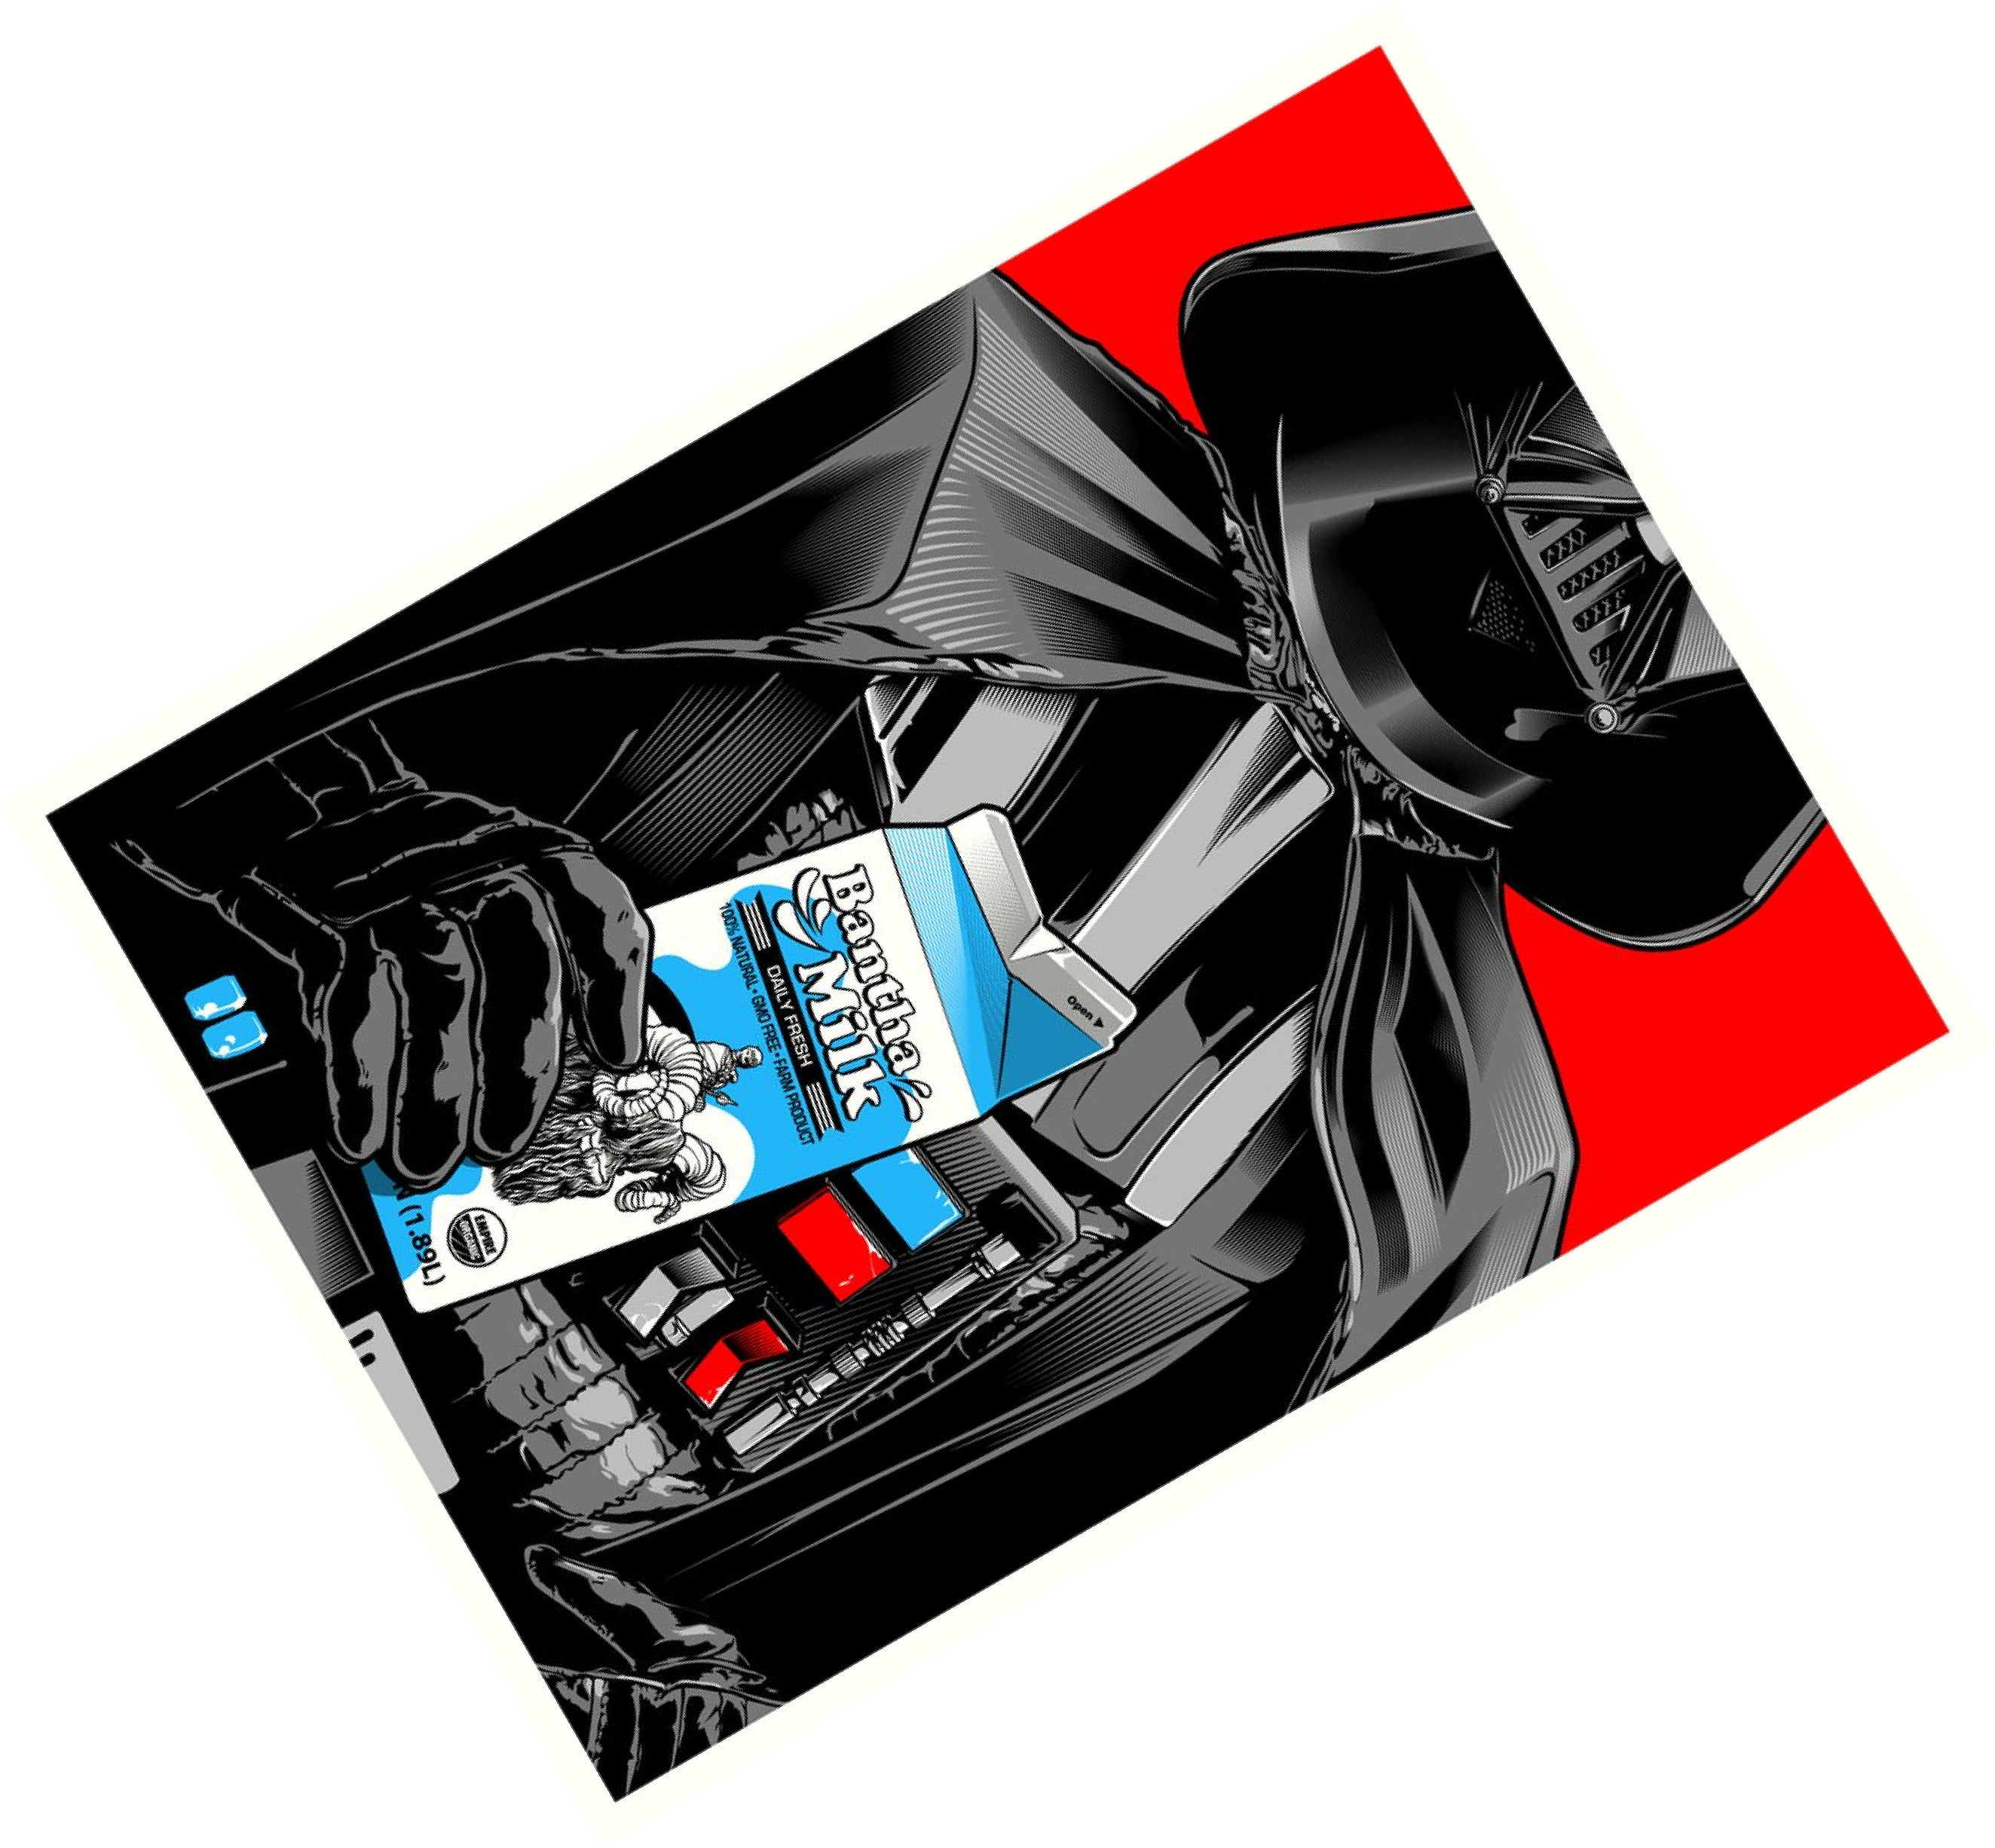
\includegraphics[width= 3.5 cm, angle = 60 ]{pop9.pdf} \end{center}

&\begin{center}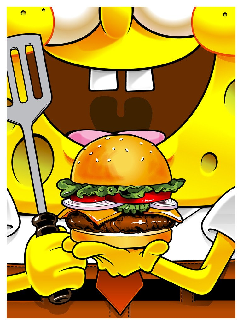
\includegraphics[width= 2.1 cm, height= 2.8 cm]{pop8.pdf} \end{center}

   &\begin{center}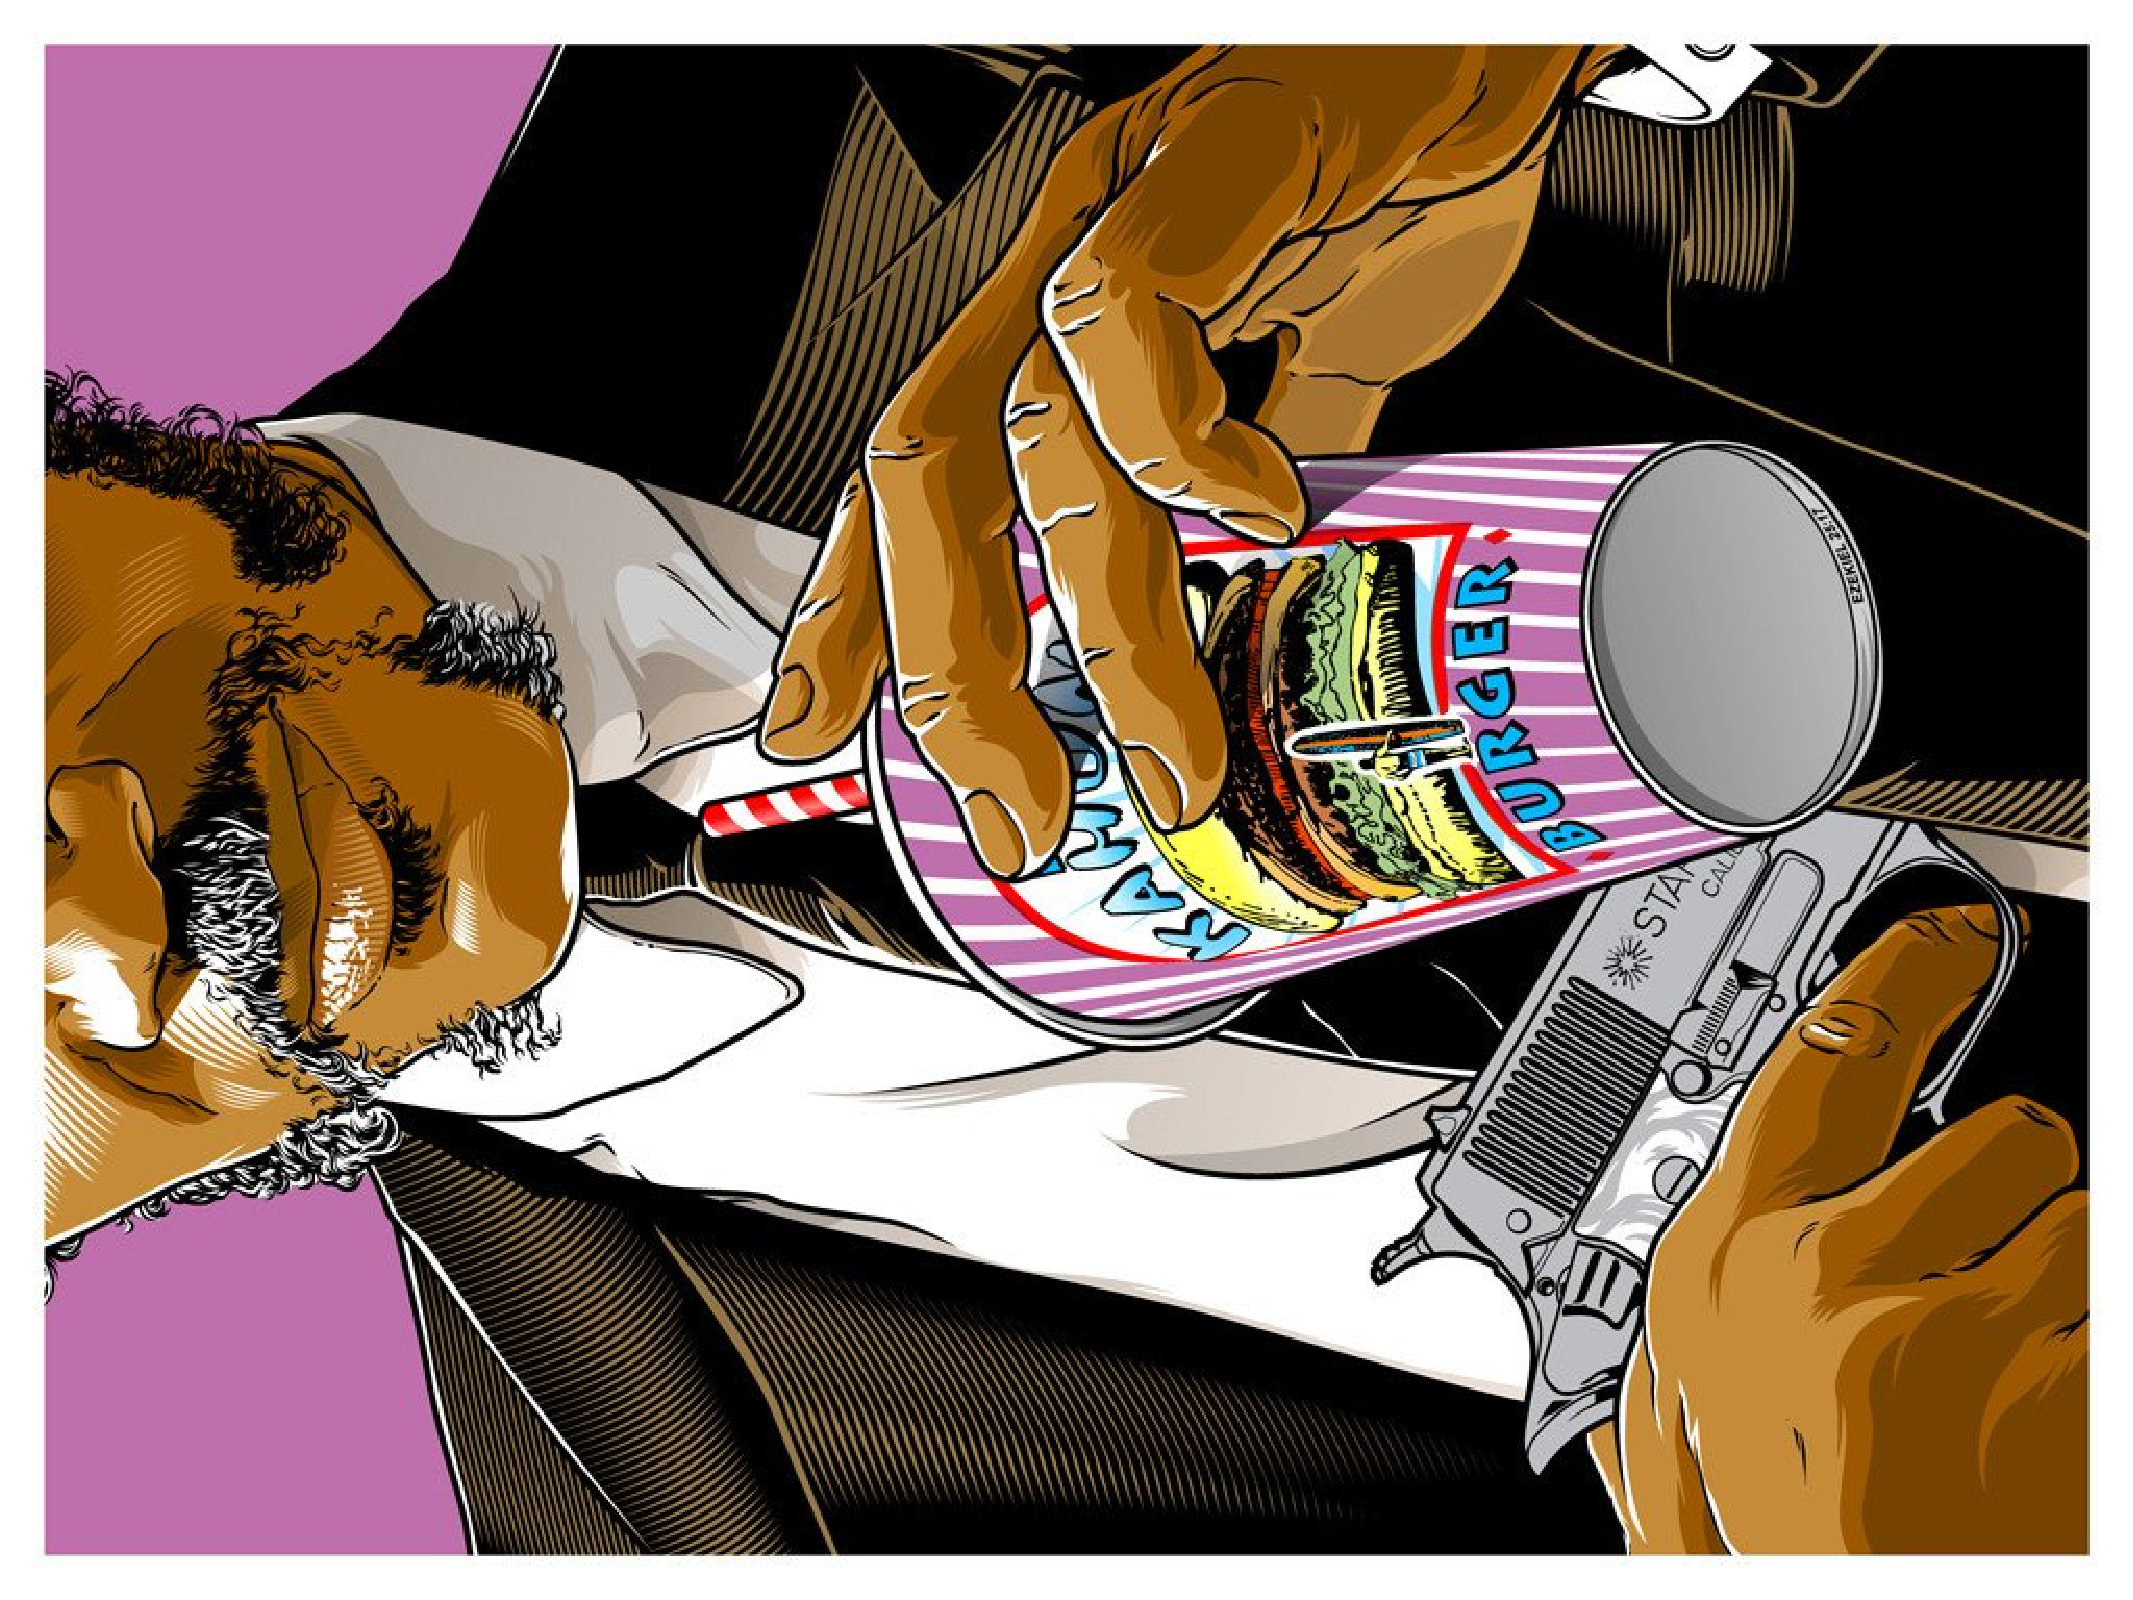
\includegraphics[angle = 270, width= 2.1 cm]{pop1.pdf}  \end{center}  \\

\end{tabular}
\caption*{Или это?}
\end{center}
\end{table}





\end{document}